\documentclass[a4paper,10pt]{article}

\usepackage{amssymb,amsmath,stmaryrd,mathrsfs}




\newtheorem{definition}{Definition}
\newtheorem{proposition}{Proposition}
\newtheorem{example}{Example}
\newtheorem{remark}{Remark}
\newtheorem{lemma}{Lemma}
\newtheorem{theorem}{Theorem}

\def\A{\ensuremath{\mathcal{A}}}
\def\C{\ensuremath{\mathcal{C}}}
\def\T{\ensuremath{\mathcal{T}}}
\def\E{\ensuremath{\mathcal{E}}}
\def\N{\ensuremath{\mathcal{N}}}
\def\bbbr{{\rm I\!R }} 
\def\bbbn{{\rm I\!N }} 
\def\idle{{\mbox{\sf idle}}} 
\def\aactive{{\mbox{\sf active}}} 
\def\error{{\mbox{\sf error}}} 
\def\TIO{{\mbox{\sf to}}} 

\newenvironment{proof}{\noindent {\it Proof. }}
{\hspace{\fill} $\blacktriangleleft$\vspace{.2cm}}

\usepackage{tikz}
\usetikzlibrary{arrows,automata,positioning}
\usetikzlibrary{automata,patterns,topaths,shapes,calc}
\tikzstyle{every picture}+=[>=stealth',initial text=]
\tikzstyle{state}=[rectangle,draw=black]

\tikzstyle{ent}=[box,draw,thick,inner sep=0pt,minimum size=2.5mm]

\title{Timed-automata \& Landing gear system ?}

\begin{document}

\maketitle

\section{Timed transition systems and Timed automata}


\subsubsection*{Timed transition system (TTS)}

A timed transition system over an alphabet $\Sigma$ (of actions) is a
transition system $\T=(S,s_0,E)$ over the set of labels $L = \Sigma
\cup \{ \varepsilon \} \cup \bbbr_{+}$ where:
\begin{itemize}
\item $S$ is a set of configurations,
\item $s_0 \in S$ is the initial configuration,
\item $E \subseteq S \times L \times S$,
\end{itemize}
such that:
\begin{itemize}
\item (Zero delay) $\forall s_1,s_2 \in S \, \, s_1 \xrightarrow{0}_{E} s_2
  \Leftrightarrow s_1=s_2$
\item (Additivity) 

$\forall s_1, s_2 ,s_3 \in S \, \, \forall d,d' \in
  \bbbr_{+} \, \, (s_1 \xrightarrow{d}_E s_2 \land s_2 \xrightarrow{d'}_E
  s_3) \Rightarrow s_1 \xrightarrow{d+d'}_E s_3$
\end{itemize}


A \emph{run} of a TTS $\T=(S,s_0,E)$ over $\Sigma$ is a sequence:
\[
s_0 \xrightarrow{d_1}_E s'_0 \xrightarrow{a_1}_E s_1
\xrightarrow{d_2}_E s'_1 \xrightarrow{a_2}_E s_2 \xrightarrow{d_3}_E \cdots
\]
starting from the initial configuration and where durations and
actions striclty alternate.


\subsubsection*{Timed automaton (TA)}

We consider a finite set $X$  of real valued variables called
clocks. These clocks evolve synchronously with time and can be reset
or compared with constant values.
For a set $X$ of clocks, $\C(X)$ denotes the set of \emph{clocks constraints}
which are conjunctions of atomic constraints of the form $x \bowtie c$
where $x \in X$, $c$ is a constant, and $\bowtie \in \{ <,\le,= , \geq,>
\}$.

We also consider a finite set $Y$ of variables over finite domains: we
write $D_y$ the finite domain of the variable $y \in Y$. 
For a set $Y$ of variables,
$\C(Y)$ denotes the set of \emph{variable constraints}
which are 
obtained by combining atomic constraints of the form $y_i = k_i$ (where
$k_i \in D_{y_i}$) with
$\lor$ and $\land$.
An update $u \in Up(Y)$ is a set of assignments of the form $y_i :=
k_i$ such that for $i \neq j$, $y_i \neq y_j$.



A timed automaton over an alphabet $\Sigma$ (of actions) is a tuple $\A=(X,Y,Q,q_0,\Delta,I)$ where:
\begin{itemize}
\item $X$ is a finite set of clocks,
%($X = \bigcup_{i=1}^{|X|} \{ x_i \in \bbbr_+ \}$),
\item $Y$ is a finite set of variables (with finite range),
\item $Q$ is a finite set of states,
\item $q_0 \in Q$ is the initial state,
\item $\Delta \subseteq Q \times \C(X) \times \C(Y) \times (\Sigma
  \cup \{ \varepsilon \}) \times \wp(X) \times Up(Y) \times Q$
\item $I : Q \to \C(X)$ (clocks invariants over states).
%\item $M : Q \to \prod_{i=1}^{|V|} D_i$ where $D_i$ is the finite
%  domain of $v_i \in V$.
\end{itemize}


Given a timed automaton $\A=(X,Y,Q,q_0,\Delta,I)$, we write $W(\A)
\subseteq Y$
the set of variables occurring in updates associated to transitions in $\Delta$.

\subsubsection*{Semantics of a timed automaton}


Given a set $X$ of clocks, a \emph{clock valuation} is a mapping $v : X \to
\bbbr_+$, with $\mathbf{0}$ the null valuation assigning zero to all
clocks in $X$. 
A valuation can be viewed as a tuple $(v(x))_{x \in X}$ defining a
point in $\bbbr_{+}^{|X|}$
(we write $\bbbr_{+}^{|X|}$ the set of valuations over $X$).
For $d \in \bbbr_+$, we write $v+d$ the valuation such
that for all $x \in X$, $(v+d)(x) = v(x) + d$. For $r \subseteq X$, we
write $v[r \mapsto 0]$ the valuation such
that for all $x \in X$, $v[r \mapsto 0](x) =0$ if $x \in r$ and $v(x)$
otherwise. Clocks constraints are interpreted on clock valuations: a
valuation $v$ satisfies the atomic constraint $x \bowtie c$, denoted by
$v \models x \bowtie c$, iff $v(x) \bowtie c$ is true. The notation is
extended to general clock constraints. 

Similarly,
given a finite set $Y$ of variables over finite domains,
a \emph{variable valuation} is a mapping $w : Y \to
\cup_{y \in Y} D_y$ (such that for all $y \in Y$, $w(y) \in D_y$).
We write $Y^D$ the set of valuations over $Y$.
Given a variable valuation $w$ and an update $u$, we write $w[u]$ the
valuation such that $w[u](y) = k$ if $y := k$ belongs to $u$, and
$w(y)$ otherwise.
Variables constraints are interpreted on variables valuations: a
valuation $w$ satisfies the atomic constraint $y=k$, denoted by
$w \models y=k$, iff $w(y) = k$ is true. The notation is
extended to general variable constraints. 



The \emph{semantics} of a timed automaton $\A=(X,Y,Q,q_0,\Delta,I)$
over an alphabet $\Sigma$ is defined from a initial variable valuation $w_0$
by a timed transition system
$\T_{\A}[w_0] = (S,s_0,E)$ over $\Sigma$ where:
\begin{itemize}
\item $S = \left \{ (q,v,w) \in Q \times \bbbr_{+}^{|X|}  \times
    Y^D \mid v \models I(q) \right \}$
\item $s_0 = (q_0,\mathbf{0},w_0)$
\item $E = \begin{array}{ll}
& \left \{ 
(q,v,w) \xrightarrow{d}_E (q,v+d,w) \mid d \in \bbbr_+ 
%\land v + d \models I(q) 
\right \} \\
\cup & 
\left \{ \begin{array}{l}
(q_1,v_1,w_1) \xrightarrow{a}_E (q_2,v_2,w_2) \mid  
\exists q_1 \xrightarrow{g_c,g_Y,a,r,u}_{\Delta} q_2 \\
v_1 \models g_c \, \land w_1 \models g_Y \, \land v_2 = v_1[r \mapsto
0] \land w_2 = w_1[u]
\end{array}
\right \}
\\
\end{array}$
\end{itemize}




\subsubsection*{Product of timed automata}

For $i \in \{ 1, \cdots , n \}$, let $\A_i = (X_i,Y_i,Q_i,i_0,\Delta_i,I_i)$ be timed automata over
$\Sigma_i$ such that for $i \neq j$, $X_i \cap X_j = \emptyset$ and
$W(\A_i) \cap W(\A_j) = \emptyset$, and
let $f$ be a partial mapping from
$\prod_{i=1}^{n} (\Sigma_i \cup \{ \varepsilon , - \})$ to
$\Sigma \cup \{ \varepsilon \}$ such that $f(-, \cdots , -)$ is not
defined. The $f$-synchronized product of $\A_i$ is defined by:
\[
\bigotimes \A_i = \left (
\bigcup X_i , \bigcup Y_i , \prod Q_i , (i_1,\cdots , i_n) , \Delta, I
\right )
\]
where:
\begin{itemize}
\item $\forall (q_1,\cdots , q_n) \in \prod Q_i \quad I((q_1,\cdots ,
  q_n)) = \bigwedge I_i(q_i)$
\item $(q_1,\cdots , q_n)  \xrightarrow{g_c,g_Y,a,r,u} (q'_1,\cdots ,
  q'_n) \in \Delta$ iff there exists a non-empty set $\N 
  \subseteq \{ 1 , \cdots n \}$ such that:
\begin{itemize}
\item $\forall j \in \N \, \, \exists q_j
  \xrightarrow{g_{c_j},g_{Y_j},a_j,r_j,u_j} q'_j \in \Delta_j$ such
  that:
\begin{itemize}
\item $g_c = \bigwedge\limits_{j \in \N} g_{c_j}$ and $g_Y = \bigwedge\limits_{j \in
    \N} g_{Y_j}$ and $r = \bigcup\limits_{j \in \N} r_j$ and $u = \bigcup\limits_{j \in \N} u_j$
\item $f(l_1,\cdots,l_n) = a$ where $l_i = -$ if $i \not \in \N$ and
  $a_i$ otherwise.
\end{itemize}
\item $\forall j \in \{ 1 , \cdots , n \} \backslash \N \quad q_j =
  q'_j$
\end{itemize}
\end{itemize}

\subsubsection*{Time-out mechanism}

Let $\A = (X,Y,Q,q_0,\Delta,I)$ be a timed automaton
over $\Sigma_L \times \Sigma_S$ where $\Sigma_L$ contains actions and
$\Sigma_S$ contains synchronization labels.
Each state $q \in Q$ can be associated to a
finite set $T_q$ of time-out mechanisms. A time-out mechanism for a state
$q$ is defined by a duration $d \in \bbbr_+$ and a property $p \in \C(Y)$
over variables and specifies that if the state $q$ is reached at time
$t$, an error state must be reached if at time $t + d$  the property
$p$ does not hold. We write $\tau = (d,p)$ such a time-out mechanism.
Each time-out mechanism $\tau=(d,p) \in T_q$ of a state $q \in Q$ is described by a timed
automaton $\A_\tau = (\{ x_\tau \},Y,Q_\tau, \idle_\tau ,
\Delta_\tau,I_\tau)$ 
over $\Sigma_\tau = \{ a_q \}$ where
$a_q$ is the synchronization label in $\Sigma_S$ associated to $q$
such that:
\begin{itemize}
\item $Q_\tau = \{ \idle_\tau, \aactive_\tau ,
\error \}$
\item $I_\tau(\idle_\tau) = I_\tau(\error) = \top$ and
  $I_\tau(\aactive_\tau) =  x_\tau \leq d$ 
\item $\Delta_\tau$ is defined by:

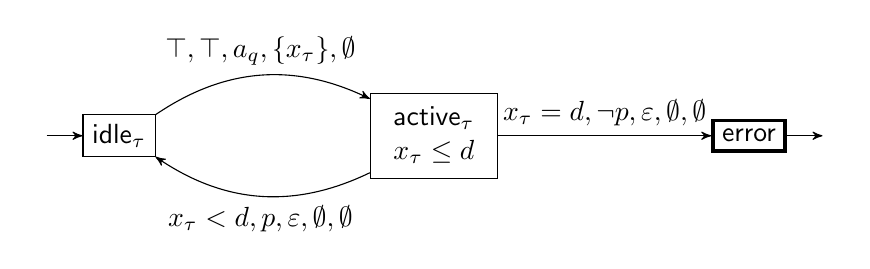
\begin{tikzpicture}[accepting/.style={very thick,accepting by arrow}]
%\tikzstyle{etiquette}=[midway,fill=black!20]
\node[state,initial] (idle) at (0,0) {$\idle_\tau$};
\node[state] (active) at (4,0) {$\begin{array}{l} \aactive_\tau \\
    x_\tau \leq d \end{array}$};
\node[state,accepting] (error) at (8,0) {$\error$};
\path[->] (idle) edge [bend right=-30] node [above]
{$\top,\top,a_q,\{x_\tau \},\emptyset$} (active)
                (active) edge [bend left=30] node [below] {$x_\tau < d
                  , p,\varepsilon,\emptyset,\emptyset$} (idle)
                (active) edge [above] node {$x_\tau=d , \neg p ,
                  \varepsilon , \emptyset , \emptyset$} (error);
\end{tikzpicture}


\end{itemize}


\subsubsection*{Time-out mechanisms over states of a timed automaton}

Let 
$\A = (X,Y,Q,q_0,\Delta,I)$ be a timed automaton over $\Sigma =
\Sigma_L \times \Sigma_S$ such that:
\begin{itemize}
\item $\Sigma_S = \{ a_q \mid q \in Q \}$
\item $\forall q_1 \xrightarrow{g_c,g_Y,(a_L,a_S),r,u} q_2 \in \Delta
  \, \, \,  a_S = a_{q_2}$
\item $T_\A = \bigcup_{q \in Q} T_q$ is the finite set of time-out
  mechanisms associated to states of $Q$:
\begin{itemize}
\item $T_q = \left \{ 
\tau_q^1 , \cdots , \tau_q^{n_q}
\right \}$ is the finite set of
  time-out mechanisms associated to the state $q$
\item each time-out mechanism $\tau$ is associated to a timed
  automaton $\A_\tau$ as described above and we write $A(T_\A)$ the
  set of timed automata associated to time-out mechanisms belonging
  to $T_\A$
%\item we write $Q_{\TIO} = \{ q \in Q \mid T_q \neq \emptyset \} \subseteq Q$
\end{itemize}
\item $f_{to}$ is the synchronization partial mapping from
$(\Sigma_L \cup \{ \varepsilon , - \}) \times (\Sigma_S  \cup \{
 - \}) \times \prod_{\tau \in T_\A} (\Sigma_\tau  \cup
\{ \varepsilon, - \})$ to $(\Sigma_L \cup \{ \varepsilon \}) \times (\Sigma_S \cup \{ \varepsilon \}) \times \prod_{\tau \in T_\A}
(\Sigma_\tau \cup \varepsilon)$ such that:
\[
\begin{array}{l}
f_{to}(l_\A,l_{\tau_1},\cdots , l_{\tau_n}) \\
=
\left \{
\begin{array}{ll}
(l_\A,l'_{\tau_1},\cdots , l'_{\tau_n}) &
\mbox{if} \, \, \left (
\begin{array}{ll} 
&  l_\A = (a_L,a_q) \land a_L \neq - \land a_S \neq - \\
\land & \forall i \, \, \tau_i \in T_q \Rightarrow
(a_q=l_{\tau_i}=l'_{\tau_i}) \\
\land & \forall i \, \, \tau_i \not \in T_q \Rightarrow
(l_{\tau_i}= - \land l'_{\tau_i} = \varepsilon) \\
\end{array} \right )
\\ 
& \mbox{or} 
\, \, \left (
\begin{array}{ll} 
&  l_\A = (-,-) \land l'_\A = (\varepsilon , \varepsilon) \\
\land & \exists j \, \, l_{\tau_j} \neq - \land \forall i \, \,
l'_{\tau_i} = \varepsilon \\
\end{array} \right )
\\
\mbox{undefined} & \mbox{otherwise}
\end{array}
\right .
\end{array}
\]
\end{itemize}
We define the timed automaton (with time-out features) as the
$f_{to}$-synchronized product:
\[
\A[T_\A] = \A \otimes \bigotimes_{\A_\tau \in A(T_\A)} \A_\tau
\]

\section{Application to the landing gear system}

\subsubsection*{Without time-out mechanisms}

(Parties noires, bleues, vertes de l'automate de Fran\c{c}ois)


The set $Y$ of variables can be partitionned as $Y = Y_L \cup Y_C \cup
Y_S$ ($Y_L$ contains variables corresponding to lights, $Y_C$ contains
variables corresponding to commands and $Y_S$ contains
variables corresponding to sensors).

The set $\Sigma$ is defined as the cartesian product $\Sigma = \Sigma_L
\times \Sigma_S$ where $\Sigma_L$ contains actions corresponding to
the modification of variables and $\Sigma_S$ contains synchronization
labels (used later for time-out mechanisms). Note that transitions
that modify variables in $Y_S$ are not guarded (the system cannot
control the data sent by sensors).


.... pour les
transitions avec un ``temps'' , par exemple $e_1 \xrightarrow{200ms}
e_2$ dans l'automate de Fran\c{c}ois (qui mod\'elise le fait que
l'on reste au moins 200ms dans l'\'etat $e_1$ avant de passer \`a
$e_2$), on peut utiliser une horloge $x_t$ et repr\'esenter cette
transition par
$\xrightarrow{\_,\_,\_,\{ x_t \} \cup \_,\_} e_1 \xrightarrow{x_t \geq 200 , \top , \varepsilon , \{ x_t \},\emptyset} e_2$
d'un automate temporis\'e.

\subsubsection*{With time-out mechanisms}

(Parties rouges de l'automate de Fran\c{c}ois)

la propriete $p$ de chaque time-out peut \^etre d\'ecoup\'ee :
disjonction   ``annulation'' , ``partie monitor\'ee''


\bibliographystyle{plain}
\bibliography{fbibli}



\end{document}